
\chapter{Wave-Particle Duality}%
\label{cha:Wave-Particle Duality}

\begin{parag}{Interference in Double slit exp.}
    \begin{center}
    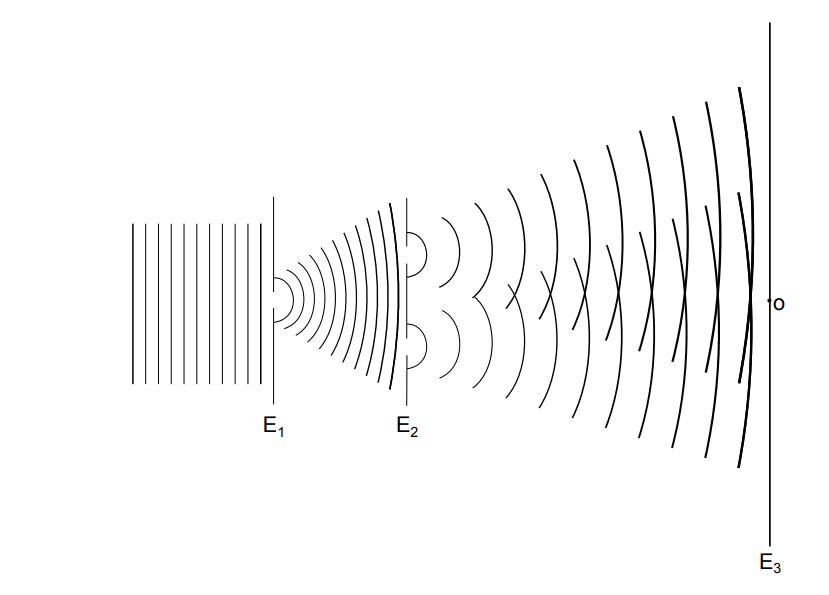
\includegraphics[scale=0.3]{screenshots/2026-09-09.png}
    \end{center}
	What this has shown is that light behaved like a wave in our case. If light were in fact particle, the result of the following experiences would be different. The resulting wave would be something like this:
	\begin{center}
	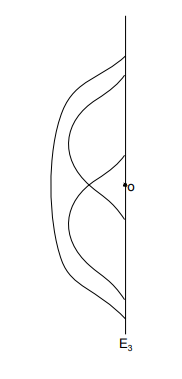
\includegraphics[scale=0.4]{screenshots/2026-09-09_1.png}
	\end{center}
	However lights behaving like a wave is something that we can all agree on, on the other case, imagine doing the same experiment but for electrons or $\text{C60}$, the resulting frequency would corresponds to a wave as for lights. And this frequency is \important{constant} i.e., we can send electrons one after the other then after collecting the statistics; remarkably the function we get is the same prediction as the one of wave.
\end{parag}
\chapter{Mathematical notions}%
\label{cha:Mathematical notions}

\subsection{Recap of linear algebra in Dirac notation}
The arena for quantum mechanics is Hilbert space (a vector space on $\mathbb{C}$).\\
$ $\\
\begin{parag}{Notation}
	The language in order to speak in quantum science is \important{Dirac} notation.
	\begin{definition}{Ket}
    \begin{align*} 
    	\vec{\phi} =  \ket{\phi} = \begin{pmatrix} \phi_1 \\ \phi_1 \\ \vdots \\ \phi_n \end{pmatrix} \mathspace \mathspace, \phi_i \in \mathbb{C}\\
    \end{align*}
	\end{definition}
	\begin{definition}{Bra}
	\begin{align*} 
		\vec{\phi}^{\dagger} = \bra{\phi} =  \left(\phi_i^\ast, \phi_2^{\ast}, \ldots, \phi_D^{\ast}\right), \phi_i \in \mathbb{C}
	\end{align*}
	\end{definition}
	Kets and Bras are the foundation of the language of quantum science, those will be used extensively throughout the whole course.
	\begin{definition}{Inner product}
	In  our new space, we will define the inner product as 
	\begin{align*} 
		\vec{\phi}^{\dagger} \cdot \vec{\phi} =  \sum_{i= 1}^{D} \phi_i^{\ast} \cdot \phi_i 
	\end{align*}
	\end{definition}
\end{parag}


\begin{parag}{Properties}
	As for vector in classical vector space, vector inside Hilbert space also end up having properties that we can use in order to prove theorems:
    \begin{align*} 
		\bra{\phi}\ket{\varphi}^{\ast} &= \bra{\varphi}\ket{\phi}\\
		\left(\alpha^\ast\bra{\phi_1} + \beta^{\ast}\bra{\phi_2}\right) \ket{\varphi} &= \alpha^\ast \bra{\phi_1}\ket{\varphi} + \beta^{\ast}\bra{\phi_2}\ket{\varphi}
    \end{align*}
	The positivity of bracket:
	\begin{align*} 
		\bra{\phi}\ket{\phi} \geq 0
	\end{align*}
	We also have triangle inequality and Cauchy-Schwartz:
	\begin{align*} 
		\left\|\phi + \varphi\right\| &\leq \left\|\phi\right\| + \left\|\varphi\right\|\\
		\left|\bra{\phi}\ket{\varphi}\right| &\leq \left\|\phi\right\|\left\|\varphi\right\|
	\end{align*}
\end{parag}


\begin{parag}{Orthonormal basis in $\mathcal{H}$}
    the dimension of our space is denoted as $\text{dim} \mathcal{H} = D$. The basis of that space is composed of basis vector which are noted as:
	\begin{align*} 
		\ket{u_1}, \ket{u_2}, \ldots, \ket{u_D}
	\end{align*}
	Where 
	\begin{align*} 
		\bra{u_i}\ket{u_j} = \begin{cases}
			1 \mathspace i = j\\ 0 \mathspace j \neq i
		\end{cases} 
	\end{align*}
	as vector that are not equal are orthogonal hence their inner product equals $0$.
	\begin{subparag}{Example}
	    The most commons space that will be used during this course is $\mathbb{C}^2 =  \left\{\begin{pmatrix} \alpha \\ \beta \end{pmatrix}, \alpha, \beta \in \mathbb{C} \right\}$. In this case we define our vector as 
		\begin{align*} 
			\ket{\phi} = \alpha \ket{0} + \beta \ket{1} 
		\end{align*}
	\end{subparag}
\end{parag}

\begin{parag}{Tensor product}
	The goal of a tensor product is to combine spaces together. 
	\begin{definition}
    Given $\mathcal{H}_1$ and $\mathcal{H}_2$ we define $\mathcal{H}_1 \otimes \mathcal{H}_2$ as
	\begin{align*} 
		\left{\ket{u_1}, \ket{u_2}, \ldots, \ket{u_{D_1}}\right} \otimes \left{\ket{v_1}, \ket{v_2}, \ldots, \ket{v_{D_2}}\right} \to \left{\ket{u_i} \otimes \ket{v_j} = \ket{u_i, v_j}\right}
	\end{align*}
	Where $i =  1, \ldots, D_1$ and $j = 1, \ldots, D_2$.
	\end{definition}
	\begin{subparag}{Example}
	    Taking again $\mathbb{C}^2$ We  want to convert it into $\mathbb{C}^2 \otimes \mathbb{C}^2$ ,the new basis of our space this gives:
		\begin{align*} 
			\ket{0} \otimes \ket{0} = \ket{ 0\; 0}\\
			\ket{0} \otimes \ket{1} = \ket{ 0\; 1}\\
			\ket{1} \otimes \ket{0} = \ket{ 1\; 0}\\
			\ket{1} \otimes \ket{1} = \ket{ 1\; 1}\\
		\end{align*}
		This allows us to have multiple qbits inside one state, which later on will allow us to have the notion of entanglement.
	\end{subparag}
	If we wanted to translate this into classical linear algebra, this result for the tensor product would be the following: given two vectors $\vec{v} =  \begin{pmatrix} \alpha \\ \beta \end{pmatrix} $ and $\vec{u} =  \begin{pmatrix} \gamma \\ \delta \end{pmatrix}$ the tensor product would be computed as 
	\begin{align*} 
		\vec{v} \otimes \vec{u} = \begin{pmatrix} \alpha\begin{pmatrix} \gamma \\\delta  \end{pmatrix}  \\ \beta \begin{pmatrix} \gamma \\\delta  \end{pmatrix}  \end{pmatrix} =  \begin{pmatrix} \alpha \gamma \\ \alpha \delta \\ \beta \gamma \\ \beta \delta \end{pmatrix} 
	\end{align*}
	\begin{subparag}{Inner product in $\mathcal{H}_1 \otimes \mathcal{H}_2$}
		\begin{align*} 
			\left(\bra{\phi_1} \otimes \bra{\phi_2}\right) \left(\ket{\phi_1} \otimes \ket{\phi_2}\right) = \bra{\phi_1}\ket{\varphi_1}\bra{\phi_2}\ket{\phi_2}
		\end{align*}
	\end{subparag}
\end{parag}



\begin{parag}{Matrix}
	\begin{definition}
    A matrix $A : \mathcal{H} \to \mathcal{H}$ is an operator defined in a given an orthonormal basis $\left\{\ket{1}, \ket{2}, \ldots, \ket{D}\right\}$ which can be represented as an $D \times D$ array where $A_{ij} =  \bra{i}A\ket{j}$. We can even define our matrix as:
	\begin{align*} 
		A =  \sum_{i, j = 1}^{D} A_{ij}\ket{i}\bra{j}
	\end{align*}
	Where $\ket{i}\bra{j}$ is the matrix that has a $1$ at the position $\left(i, j\right)$ and $0$ everywhere else.
 	\end{definition}
	\begin{subparag}{Tensor product of matrices}
	    Given two Hilbert spaces $\mathcal{H}_1, \mathcal{H}_2$ we know how to compute the inner product space of the tensor product between our two spaces $\mathcal{H}_1, \mathcal{H}_2$ as seen before. What we want to see now is the tensor product between two matrices $A$ and $B$.\\
		$ $\\
		To do so we'll use the definition of the matrix using the '\textit{ket bra}' notation of the definition above.
		\begin{align*} 
			A \otimes B = \sum_{i, j, j, l} A_{ij} B_{jl } \underbrace{\ket{i}\bra{j}  \otimes \ket{k}\bra{l}}_{\left(\ket{i} \otimes \ket{k}\right)\left(\bra{j} \otimes \bra{l}\right)}
		\end{align*}
		\begin{framedremark}
		The notation $\ket{i} \otimes \ket{k}$ can be simplified by $\ket{i, k}$.
		\end{framedremark}
		\begin{align*} 
			A \otimes B &= \sum_{i, j = 1}^{D_1}\sum_{k, l}^{D_2} A_{ijkl} \ket{i, k} \bra{j, l}\\
		\end{align*}
		The resulting dimension of our matrix is given by $D_1D_2 \times D_1 D_2$ where
		\begin{align*} 
			 \left(A \otimes B\right)_{ik, jl} =  A_{ij} B_{kl}
		\end{align*}
	\end{subparag}
	\begin{subparag}{Example}
	    Given the product of $\mathbb{C}^2 \otimes \mathbb{C}^2$, let us see what would be the tensor product of the two matrices:
		\begin{align*} 
			A = \begin{pmatrix} a & b \\ c & d \end{pmatrix}   \mathspace \mathspace B = \begin{pmatrix} e & f \\ g & h \end{pmatrix} 
		\end{align*}
		The goal is to compute $A \otimes B$.
		\begin{align*} 
			A \otimes B &=  \begin{pmatrix} a & b \\ c & d \end{pmatrix} \otimes \begin{pmatrix} e & f \\ g & h \end{pmatrix} \\
											 &= \begin{pmatrix} a \cdot B & b B \\ c B & d B \end{pmatrix} \\
											 &= \begin{pmatrix} ae & af & be & bf \\ ad & ah & bd & bh \\ ce & cf & ge & gf \\ cd & ch & gd & gh \end{pmatrix} 
		\end{align*}
	\end{subparag}

\end{parag}


\subsection{Hermitian matrix}
First let us do some notation:
\begin{align*} 
	A^{\dagger} &=  \sum_{i, j} A_{ij}^{\ast} \ket{j}\bra{i} \\
	&= \sum_{i, j} A_{ij}^{\ast} \ket{i}\bra{j}
\end{align*}
We have the following:
\begin{align*} 
	\left(A^{\ast}\right)_{ij} = A^{\ast}_{ij}
\end{align*}
\begin{parag}{Hermitiam matrices}
    \begin{definition}
    An Hermitian matrix is a given operator $A$ on an Hilbert space $\mathcal{H}$ where 
	\begin{align*} 
		A = A^{\dagger} 
	\end{align*}

    \end{definition}
\end{parag}


\begin{parag}{Unitary matrices}
    
	\begin{definition}
	An unitary matrix is an Hermitian operator $U$ on an Hilbert space $\mathcal{H}$ where 
	\begin{align*} 
		U^{-1} =  U^{\dagger} 
	\end{align*}
	\end{definition}
	Here an equivalent property can be derived
	\begin{align*} 
		U U^{\dagger} =  U^{\dagger} U = I  
	\end{align*}
	Which is equivalent to say for two any given pure states $\ket{\phi}, \ket{\varphi}$
	\begin{align*} 
		\bra{\phi}\ket{\varphi} = \bra{\phi} U U^{\dagger} \ket{\varphi} =  \left(U \ket{\phi}\right)^{\dagger} \cdot \left(U \ket{\varphi}\right) 
	\end{align*}
\end{parag}


\begin{parag}{Spectral theorem for Hermitian matrices}
    \begin{theoreme}
    Given a Hermitian matrices $A$ we have that all eigenvalues of our matrix are real number where their respective eigenvector are orthonormal.
	\begin{align*} 
		A \ket{u_i} =  \lambda_i  \ket{u_i}
	\end{align*}
	with $\lambda_i \in \mathbb{R}$.\\
	$ $\\
	In particular, we have:
	\begin{align*} 
		A = \sum_{i= 1}^{d} \lambda_i \ket{v_i}\bra{v_i} 
	\end{align*}

    \end{theoreme}
\end{parag}






